% !TeX root = ../index.tex
\chapter{Database Connectivity \& Testing}
\graphicspath{{8-db-testing/images/}}

\section{Exercise 1}

\url{https://intweb.bucks.ac.uk/~21606555/oos/8-db-testing/ex1.php}

\captionsetup{type=figure}\captionof{figure}{ex1.php}
\subfile{pyg/src/8-db-testing/ex1}

\begin{figure}[H]
  \caption{Lotto numbers output}
  \centering
  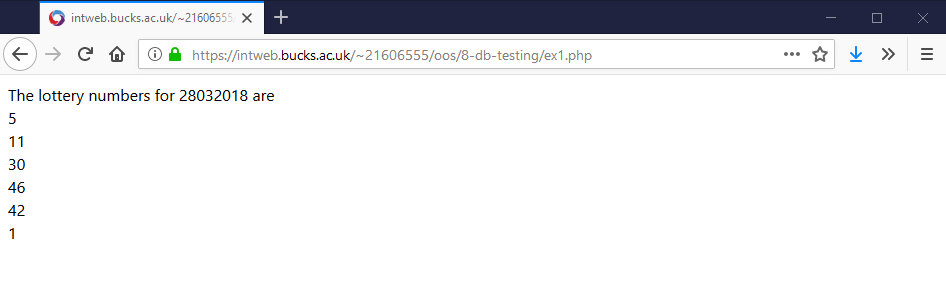
\includegraphics[width=\textwidth]{ex1-1}
\end{figure}

\begin{figure}[H]
  \caption{Checking randomness}
  \centering
  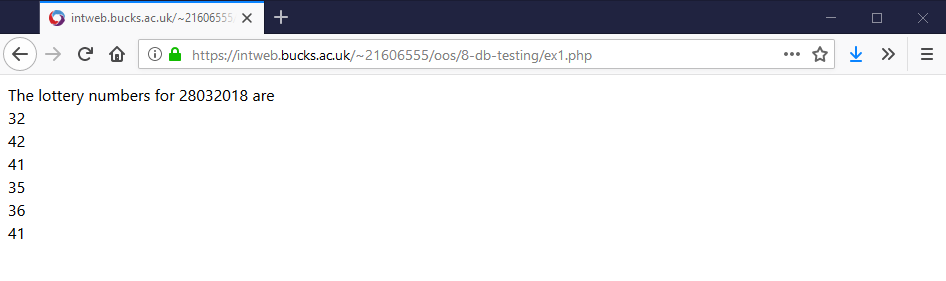
\includegraphics[width=\textwidth]{ex1-2}
\end{figure}

\section{Exercise 2}

\begin{figure}[H]
  \caption{Lotto table created}
  \centering
  \includegraphics[width=\textwidth]{ex2}
\end{figure}

\clearpage
\section{Exercise 3}

\url{https://intweb.bucks.ac.uk/~21606555/oos/8-db-testing/ex3.php}

\captionsetup{type=figure}\captionof{figure}{ex3.php}
\subfile{pyg/src/8-db-testing/ex3}

\begin{figure}[H]
  \caption{Lotto numbers and saving to database}
  \centering
  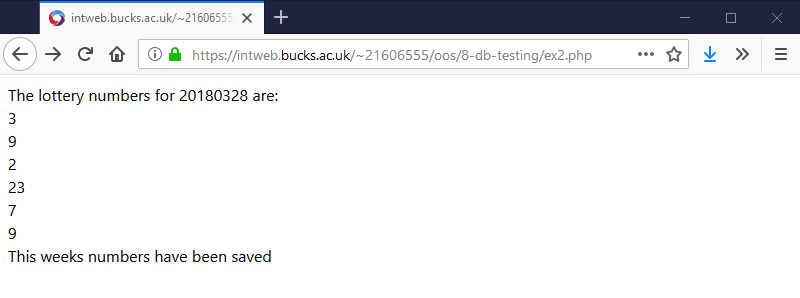
\includegraphics[width=\textwidth]{ex3-numbers}
\end{figure}

\begin{figure}[H]
  \caption{Data in database}
  \centering
  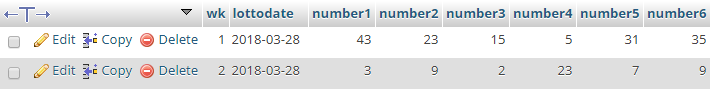
\includegraphics[width=\textwidth]{ex3-db}
\end{figure}

\clearpage
\section{Exercise 4}

\url{https://intweb.bucks.ac.uk/~21606555/oos/8-db-testing/ex4.php}

\captionsetup{type=figure}\captionof{figure}{ex4.php}
\subfile{pyg/src/8-db-testing/ex4}

\begin{figure}[H]
  \caption{Selecting from weeks in database}
  \centering
  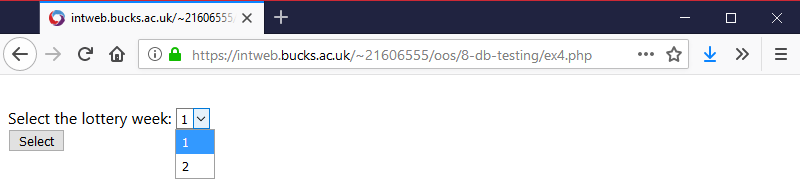
\includegraphics[width=\textwidth]{ex4-select}
\end{figure}

\begin{figure}[H]
  \caption{Displaying lotto numbers from the selected week}
  \centering
  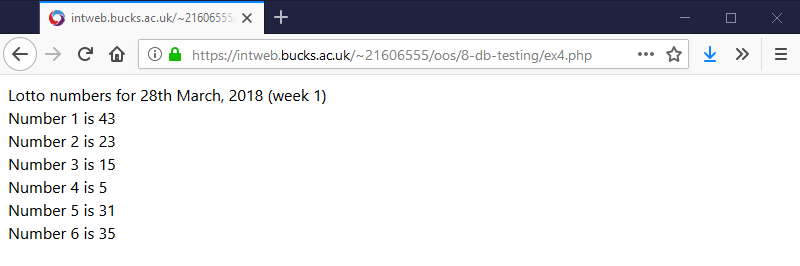
\includegraphics[width=\textwidth]{ex4-result}
\end{figure}

\clearpage
\section{Exercise 5}

\begin{figure}[H]
  \caption{Design for the lotto results page with navigation to prev/next week}
  \centering
  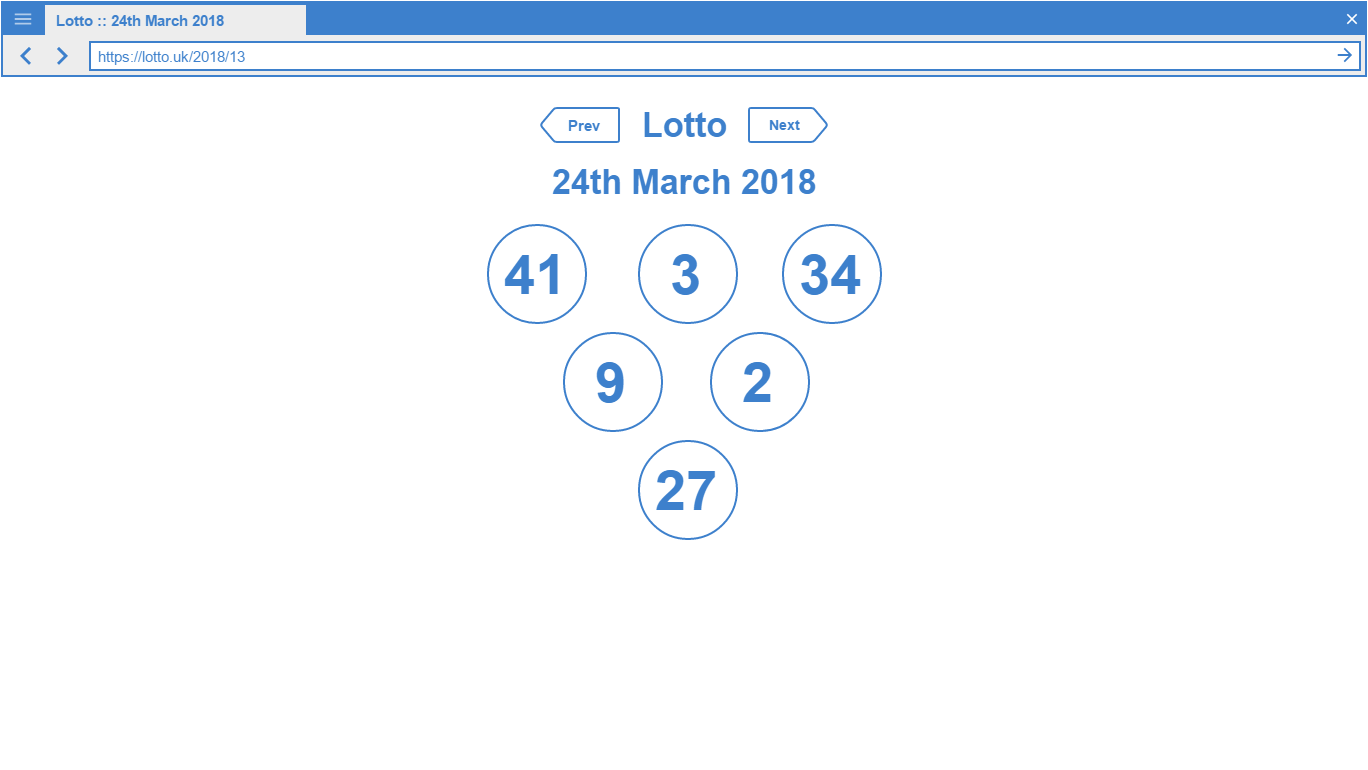
\includegraphics[width=\textwidth]{ex5}
\end{figure}
